% Hoja cuadriculada para simular apuntes a mano. Se incluye desde apuntes.tex.
\usetikzlibrary{calc,decorations.pathmorphing,arrows.meta}
\usepackage{newunicodechar}
\newunicodechar{ó}{\accent1 o}
\newunicodechar{ü}{\accent4 u}
\newunicodechar{Ó}{\accent1 O}
\newunicodechar{Í}{\accent1 I}
\definecolor{Boligrafo}{HTML}{1E3A8A}
\definecolor{KalaTinta}{HTML}{0F766E}
\definecolor{Titulo}{HTML}{B42318}
\definecolor{ResaltaDef}{HTML}{C9F2D8}
\definecolor{ResaltaRes}{HTML}{FFD8B8}
\definecolor{Cuadricula}{HTML}{BCD3EA}
\definecolor{Margen}{HTML}{D9534F}
\definecolor{Lapiz}{HTML}{6B6B6B}
\definecolor{Resaltador}{HTML}{FFF1A8}
\pagestyle{empty}
\setlength{\parskip}{0pt}

\newlength{\Celda}\setlength{\Celda}{5mm}
\newlength{\XMargen}\setlength{\XMargen}{22mm}
\newlength{\XTexto}\setlength{\XTexto}{25mm}
\newcounter{fila}
\newcommand{\PrimeraFila}{6}
\newcommand{\UltimaFila}{56}

\AddToHook{shipout/background}{%
  \begin{tikzpicture}[remember picture,overlay]
    \draw[Cuadricula,line width=.25pt,step=\Celda]
      (current page.south west) grid (current page.north east);
    \draw[Margen,line width=.7pt]
      ($(current page.north west)+(\XMargen,0)$) -- ($(current page.south west)+(\XMargen,0)$);
  \end{tikzpicture}}

\newcommand{\Mano}{\fontfamily{augie}\selectfont}
\newcommand{\g}[1]{\KalaSimbolo[1.6em]{#1}}

\newlength{\SubirFila}\setlength{\SubirFila}{0pt}
\newcommand{\EnFila}[3]{%
  \tikz[remember picture,overlay]
    \node[anchor=base west,inner sep=0pt,text=Boligrafo,font=\Mano]
      at ($(current page.north west)+(#1,-\value{fila}\Celda+1.2mm+\SubirFila)$) {#2#3};}

\newcommand{\AvanzarFila}[1][1]{%
  \addtocounter{fila}{#1}%
  \ifnum\value{fila}>\UltimaFila\relax
    \clearpage\mbox{}\setcounter{fila}{\PrimeraFila}%
  \fi}

\newcommand{\Marca}[1]{%
  \tikz[remember picture,overlay]
    \node[anchor=base,inner sep=0pt]
      at ($(current page.north west)+(\XMargen/2+1.5mm,-\value{fila}\Celda+1.2mm+\SubirFila)$) {#1};}

% \F[sangría en celdas]{margen}{contenido}
\newcommand{\F}[3][0]{%
  \AvanzarFila
  \Marca{#2}%
  \EnFila{\dimexpr\XTexto+#1\Celda\relax}{}{#3}}

% \FT: línea alta (fracciones, integrales); ocupa dos filas
\newcommand{\FT}[3][0]{%
  \AvanzarFila[2]%
  \setlength{\SubirFila}{2.5mm}%
  \Marca{#2}%
  \EnFila{\dimexpr\XTexto+#1\Celda\relax}{}{#3}%
  \setlength{\SubirFila}{0pt}}

% Fila en blanco
\newcommand{\B}[1][1]{\AvanzarFila[#1]}

% Anotación en lápiz, añadida después de clase
\newcommand{\lapiz}[1]{{\color{Lapiz}#1}}
% Tachado a mano
\newcommand{\tachar}[1]{\tikz[baseline=(t.base)]{\node[inner sep=0pt](t){#1};
  \draw[Boligrafo,line width=.6pt,decorate,decoration={random steps,segment length=2pt,amplitude=.4pt}]
  (t.west) -- (t.east);}}
% Subrayado ondulado: palabra candidata a signo
\newcommand{\candidata}[1]{\tikz[baseline=(t.base)]{\node[inner sep=0pt](t){#1};
  \draw[Boligrafo,line width=.4pt,decorate,decoration={snake,amplitude=.5pt,segment length=3pt}]
  ([yshift=-1.2pt]t.south west) -- ([yshift=-1.2pt]t.south east);}}
% Número en círculo para referencias con Ver
\newcommand{\nota}[1]{\tikz[baseline=(n.base)]\node[draw=Boligrafo,circle,inner sep=.6pt,font=\scriptsize\Mano,text=Boligrafo](n){#1};}
\newcommand{\resaltar}[1]{\tikz[baseline=(t.base)]\node[fill=Resaltador,inner sep=1pt](t){#1};}
\newcommand{\definido}[1]{\tikz[baseline=(t.base)]\node[fill=ResaltaDef,inner sep=1pt,rounded corners=1pt](t){#1};}
\newcommand{\resumen}[1]{\tikz[baseline=(t.base)]\node[fill=ResaltaRes,inner sep=1.2pt,rounded corners=1pt](t){#1};}

% \Dibujo{filas}{código tikz}: origen arriba a la izquierda del área de texto, unidades en mm
\newcommand{\Dibujo}[2]{%
  \ifnum\numexpr\value{fila}+#1\relax>\UltimaFila\relax
    \clearpage\mbox{}\setcounter{fila}{\PrimeraFila}\fi
  \begin{tikzpicture}[remember picture,overlay,x=1mm,y=-1mm,
      shift={($(current page.north west)+(\XTexto,-\value{fila}\Celda-1mm)$)},
      Boligrafo,line width=.6pt,line cap=round,font=\Mano]
    #2
  \end{tikzpicture}%
  \addtocounter{fila}{#1}}

% \Clase{curso}{fecha}{tema}
\newcommand{\Clase}[3]{%
  \clearpage\mbox{}%
  \setcounter{fila}{3}%
  \EnFila{\XTexto}{}{\Large\color{Titulo}#1}%
  \tikz[remember picture,overlay]\node[anchor=base east,inner sep=0pt,text=Titulo,font=\Mano]
    at ($(current page.north east)+(-12mm,-3\Celda+1.2mm)$) {#2};%
  \setcounter{fila}{4}%
  \EnFila{\XTexto}{}{\color{Titulo}\underline{#3}}%
  \setcounter{fila}{5}}
